\documentclass[a4paper]{article}
\usepackage[english]{babel}
\usepackage{tipa}
\usepackage{graphicx}
\usepackage{float}

\title{NLP Final Project : \\
Building an International Phonetic Alphabet Classifier}
\author{Viona Lam, Szeyin Lee}
\date{\today}

\begin{document}

\maketitle


\section{Introduction}
Given a word in its IPA form that is either English, Chinese or Japanese, our model classifies which language it is based on labeled data.

\section{Experimental Setup}

\subsection{Models}

Instead of coding the models ourselves from scratch, we leverage the existing models that have been built and optimized, available in the Stanford JavaNLP Classifier library\footnote{http://nlp.stanford.edu/software/classifier.shtml}. A classifier is a machine learning tool that takes data points and classify them into one of k classes. For this project, we are using two classifiers: Naive Bayes Model and Multinomial Logistic Regression Model. For both of the models, we use the same set of features: unigram, bigram, trigram, and counts. 

\subsubsection{Model 1: Naive Bayes (NB)}

Naive Bayes is a generative model that models the joint distribution of p(label, features). It is important to note that it has the naive Bayes assumption that the features are independent given the class.

\subsubsection{Model 2: Multinomial Logistic Regression (MLR)}
Multinomial Logistic Regression is a discriminative model. It models the
conditional distribution p(label|features) directly and does not have the strong independent assumptions as Naive Bayes.

\subsection{Data}

\subsubsection{English Data}
English data of 44,460 of the most common words from the NY Times was obtained from the Bag of Words Dataset provided by UC Irvine\footnote{\textbf{Bag of Words Data Set:} https://archive.ics.uci.edu/ml/datasets/Bag+of+Words}. These were then converted into IPA form using Tom Brondstod's English to IPA converter.\footnote{\textbf{English to IPA Converter 1:} http://tom.brondsted.dk/text2phoneme/} To ensure accuracy, the results were also partially cross-checked with another converter.\footnote{\textbf{English to IPA Converter 2: }http://lingorado.com/ipa/} In addition, as English speakers, the IPA sounded right to us.

\subsubsection{Mandarin Chinese Data}
Mandarin Chinese data of 61,698 of the most common words was obtained from the Modern Chinese Frequent Vocab List\footnote{\textbf{Modern Chinese Frequent Vocab List: }http://vdisk.weibo.com/s/ueoM8g6c-sm2o (click the blue button with the downwards arrow to download)} a text published by the People's Republic of China's State Language Commission in November 2008. These were then converted into pinyin using the NJStar software\footnote{\textbf{Chinese Word Processor: }http://www.njstar.com/cms/njstar-chinese-word-processor-download}, and then into IPA form by referring to available documentation\footnote{\textbf{Pinyin to IPA Mapping:} https://github.com/cburgmer/cjklib/blob/master/cjklib/data/pinyinipamapping.csv} from cjklib\footnote{\textbf{CJKLib: }https://code.google.com/p/cjklib/}, a publicly accessible python library. Tones were stripped from the conversions, as they would make the decision of whether a word is Chinese or not incredibly trivial. The results were partially cross-checked with another converter\footnote{\textbf{Limited Chinese to IPA Converter: }http://easypronunciation.com/en/chinese-pinyin-phonetic-transcription-converter} to ensure accuracy.

\subsubsection{Japanese Data}
Japanese Data of 123,332 of the most common words was obtained from a selection of Japanese novels online\footnote{\textbf{Most Common Words in Japanese Novels:} http://pomax.nihongoresources.com/index.php?entry=1222520260}, as processed by Michiel Kamermans. These were then converted into IPA form by referring to available documentation\footnote{\textbf{Katakana to IPA mapping: }http://en.wikipedia.org/wiki/Transcription\_into\_Japanese}\footnote{\textbf{Additional Japanese IPA information: }http://en.wikipedia.org/wiki/Help:IPA\_for\_Japanese} and our understanding of the nature of how Japanese characters are represented\footnote{\textbf{Regarding Katakana to IPA: }The data set contained the words in their original forms, as well as parsed Katakana representations. As Katakana is a Japanese syllabary, it is not complicated to convert from Katakana to IPA. The hardest part was getting Windows to cooperate with UTF-8.}. To maintain the equal distribution of sample data from each language, we randomly selected 60,000 from the processed data to operate on.


\subsection{Evaluation}
For all datasets, we randomized the data, reserve 10\% as the testing set, and train the models with the remaining 90\% data points. We compared the label output from both Naive Bayes and Multinomial Logistic Regression models, with the known label from testing set. The baseline is 33.33\% (correct by guessing randomly one of the three languages).

\section{Results}
Having earlier done a smaller scale study\footnote{\textbf{Status Report:} https://github.com/violxy/nlpfinal/blob/master/StatusReport.txt} where we obtained 98\% accuracy, we were looking to improve by using more data, and did so by using the above-mentioned data sets.\\
\\On the larger data set, with all three langauges and an overall of 155,588 training examples, and 16,570 testing examples, we obtained 99.58\% accuracy for the Naive Bayes model, and 99.70\% for the Multinomial Logistic Regression model. Our results are significantly above baseline of 33\% and almost approaches 100\%.\\

Our results are:
\begin{figure}[H]
\centering
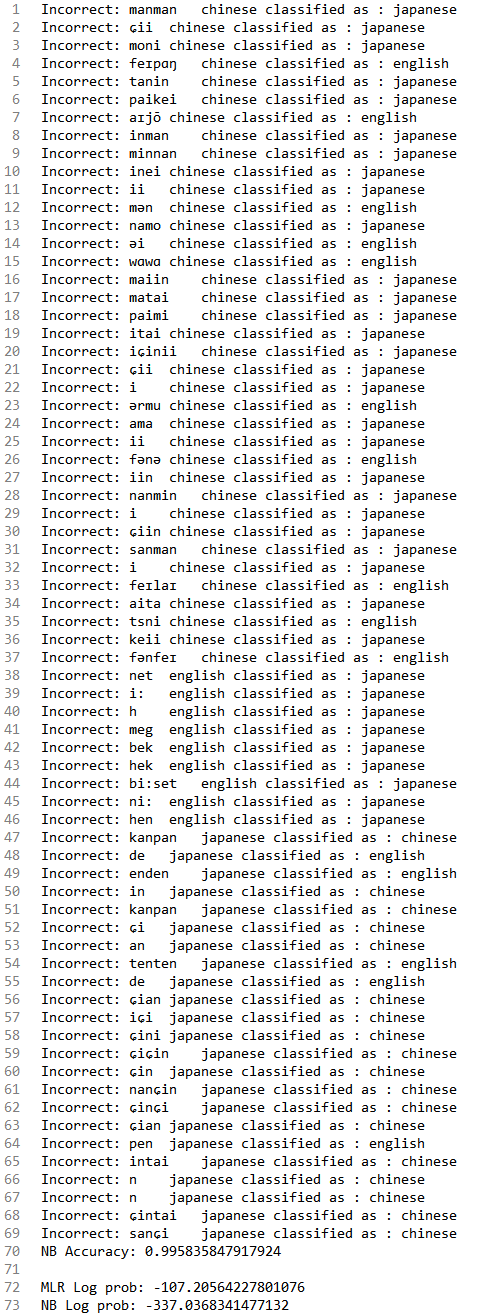
\includegraphics[width=\textwidth]{nbresult.png}
\end{figure}
\begin{figure}[H]
\centering
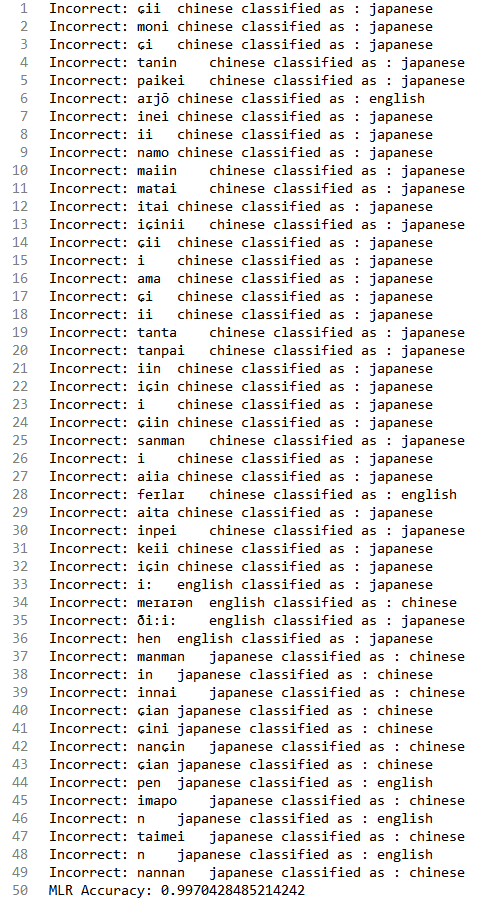
\includegraphics[width=\textwidth]{mlrresult.png}
\end{figure}
\begin{figure}[H]
\centering
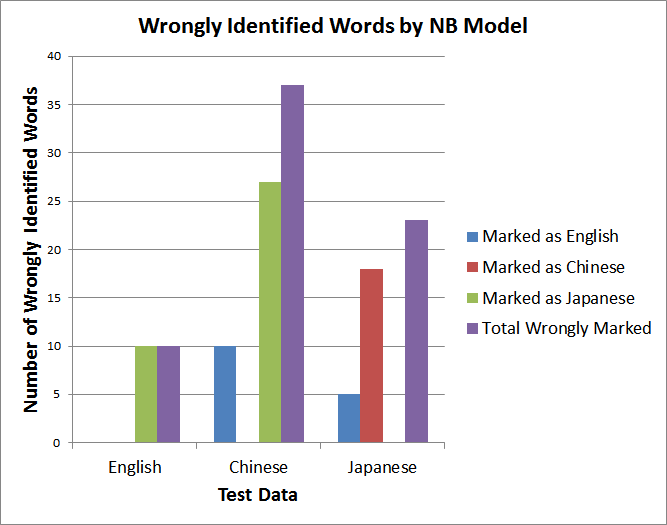
\includegraphics[width=\textwidth]{nbgraph.png}
\end{figure}
\begin{figure}[H]
\centering
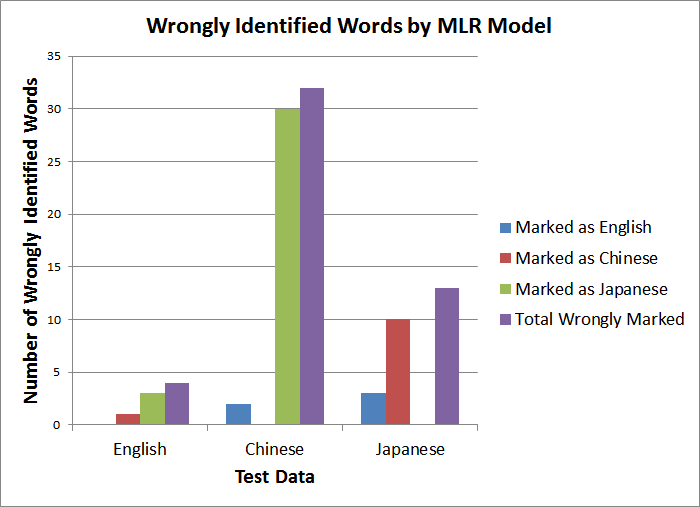
\includegraphics[width=\textwidth]{mlrgraph.png}
\end{figure}

As can be seen, most of these errors come from mistakenly classifying Chinese as Japanese, and vice versa. This makes sense, considering how close some Japanese words are to Chinese words, having partially originated from there. Furthermore, the phonemes used in Japanese do have a large overlap with those of Chinese.
\section{Conclusion}
It is possible to differentiate between languages using simple linear classifiers such as Naive Bayes and Multinomial Logistic Regression. Given more time and easier access to IPA converters, we could expand this project to other languages.\\

\section{Code}
The code for this project can be found at the shared Github repository.\footnote{\textbf{Github Repository: }https://github.com/violxy/nlpfinal/}
\end{document}